% Options for packages loaded elsewhere
\PassOptionsToPackage{unicode}{hyperref}
\PassOptionsToPackage{hyphens}{url}
\PassOptionsToPackage{dvipsnames,svgnames,x11names}{xcolor}
%
\documentclass[
  letterpaper,
]{article}

\usepackage{amsmath,amssymb}
\usepackage{iftex}
\ifPDFTeX
  \usepackage[T1]{fontenc}
  \usepackage[utf8]{inputenc}
  \usepackage{textcomp} % provide euro and other symbols
\else % if luatex or xetex
  \usepackage{unicode-math}
  \defaultfontfeatures{Scale=MatchLowercase}
  \defaultfontfeatures[\rmfamily]{Ligatures=TeX,Scale=1}
\fi
\usepackage{lmodern}
\ifPDFTeX\else  
    % xetex/luatex font selection
\fi
% Use upquote if available, for straight quotes in verbatim environments
\IfFileExists{upquote.sty}{\usepackage{upquote}}{}
\IfFileExists{microtype.sty}{% use microtype if available
  \usepackage[]{microtype}
  \UseMicrotypeSet[protrusion]{basicmath} % disable protrusion for tt fonts
}{}
\makeatletter
\@ifundefined{KOMAClassName}{% if non-KOMA class
  \IfFileExists{parskip.sty}{%
    \usepackage{parskip}
  }{% else
    \setlength{\parindent}{0pt}
    \setlength{\parskip}{6pt plus 2pt minus 1pt}}
}{% if KOMA class
  \KOMAoptions{parskip=half}}
\makeatother
\usepackage{xcolor}
\setlength{\emergencystretch}{3em} % prevent overfull lines
\setcounter{secnumdepth}{-\maxdimen} % remove section numbering
% Make \paragraph and \subparagraph free-standing
\ifx\paragraph\undefined\else
  \let\oldparagraph\paragraph
  \renewcommand{\paragraph}[1]{\oldparagraph{#1}\mbox{}}
\fi
\ifx\subparagraph\undefined\else
  \let\oldsubparagraph\subparagraph
  \renewcommand{\subparagraph}[1]{\oldsubparagraph{#1}\mbox{}}
\fi

\providecommand{\tightlist}{%
  \setlength{\itemsep}{0pt}\setlength{\parskip}{0pt}}\usepackage{longtable,booktabs,array}
\usepackage{calc} % for calculating minipage widths
% Correct order of tables after \paragraph or \subparagraph
\usepackage{etoolbox}
\makeatletter
\patchcmd\longtable{\par}{\if@noskipsec\mbox{}\fi\par}{}{}
\makeatother
% Allow footnotes in longtable head/foot
\IfFileExists{footnotehyper.sty}{\usepackage{footnotehyper}}{\usepackage{footnote}}
\makesavenoteenv{longtable}
\usepackage{graphicx}
\makeatletter
\def\maxwidth{\ifdim\Gin@nat@width>\linewidth\linewidth\else\Gin@nat@width\fi}
\def\maxheight{\ifdim\Gin@nat@height>\textheight\textheight\else\Gin@nat@height\fi}
\makeatother
% Scale images if necessary, so that they will not overflow the page
% margins by default, and it is still possible to overwrite the defaults
% using explicit options in \includegraphics[width, height, ...]{}
\setkeys{Gin}{width=\maxwidth,height=\maxheight,keepaspectratio}
% Set default figure placement to htbp
\makeatletter
\def\fps@figure{htbp}
\makeatother
% definitions for citeproc citations
\NewDocumentCommand\citeproctext{}{}
\NewDocumentCommand\citeproc{mm}{%
  \begingroup\def\citeproctext{#2}\cite{#1}\endgroup}
\makeatletter
 % allow citations to break across lines
 \let\@cite@ofmt\@firstofone
 % avoid brackets around text for \cite:
 \def\@biblabel#1{}
 \def\@cite#1#2{{#1\if@tempswa , #2\fi}}
\makeatother
\newlength{\cslhangindent}
\setlength{\cslhangindent}{1.5em}
\newlength{\csllabelwidth}
\setlength{\csllabelwidth}{3em}
\newenvironment{CSLReferences}[2] % #1 hanging-indent, #2 entry-spacing
 {\begin{list}{}{%
  \setlength{\itemindent}{0pt}
  \setlength{\leftmargin}{0pt}
  \setlength{\parsep}{0pt}
  % turn on hanging indent if param 1 is 1
  \ifodd #1
   \setlength{\leftmargin}{\cslhangindent}
   \setlength{\itemindent}{-1\cslhangindent}
  \fi
  % set entry spacing
  \setlength{\itemsep}{#2\baselineskip}}}
 {\end{list}}
\usepackage{calc}
\newcommand{\CSLBlock}[1]{\hfill\break\parbox[t]{\linewidth}{\strut\ignorespaces#1\strut}}
\newcommand{\CSLLeftMargin}[1]{\parbox[t]{\csllabelwidth}{\strut#1\strut}}
\newcommand{\CSLRightInline}[1]{\parbox[t]{\linewidth - \csllabelwidth}{\strut#1\strut}}
\newcommand{\CSLIndent}[1]{\hspace{\cslhangindent}#1}

% TODO: Add custom LaTeX header directives here

%\usepackage{ulem}
\usepackage{amsmath}
\usepackage{xcolor}
\usepackage{graphicx} 
\usepackage{fancyhdr} 
%\usepackage{wallpaper}
%  - \usepackage[page,toc,titletoc,title]{appendix}
\pagestyle{fancy} 
%  - \usepackage{float}
%  - \floatplacement{table}{H}

\setlength\headheight{28pt}
\addtolength{\headwidth}{\marginparsep}
\addtolength{\headwidth}{\marginparwidth}
\addtolength{\headwidth}{0.3cm}

\lhead{\leftmark}
\rhead{\includegraphics[width=0.5cm]{../../images/mm_stamp_small_alpha.png}}
\makeatletter
\@ifpackageloaded{caption}{}{\usepackage{caption}}
\AtBeginDocument{%
\ifdefined\contentsname
  \renewcommand*\contentsname{Table of contents}
\else
  \newcommand\contentsname{Table of contents}
\fi
\ifdefined\listfigurename
  \renewcommand*\listfigurename{List of Figures}
\else
  \newcommand\listfigurename{List of Figures}
\fi
\ifdefined\listtablename
  \renewcommand*\listtablename{List of Tables}
\else
  \newcommand\listtablename{List of Tables}
\fi
\ifdefined\figurename
  \renewcommand*\figurename{Figure}
\else
  \newcommand\figurename{Figure}
\fi
\ifdefined\tablename
  \renewcommand*\tablename{Table}
\else
  \newcommand\tablename{Table}
\fi
}
\@ifpackageloaded{float}{}{\usepackage{float}}
\floatstyle{ruled}
\@ifundefined{c@chapter}{\newfloat{codelisting}{h}{lop}}{\newfloat{codelisting}{h}{lop}[chapter]}
\floatname{codelisting}{Listing}
\newcommand*\listoflistings{\listof{codelisting}{List of Listings}}
\makeatother
\makeatletter
\makeatother
\makeatletter
\@ifpackageloaded{caption}{}{\usepackage{caption}}
\@ifpackageloaded{subcaption}{}{\usepackage{subcaption}}
\makeatother

\usepackage{hyphenat}
\usepackage{ifthen}
\usepackage{calc}
\usepackage{calculator}



\usepackage{graphicx}
\usepackage{geometry}
\usepackage{afterpage}
\usepackage{tikz}
\usetikzlibrary{calc}
\usetikzlibrary{fadings}
\usepackage[pagecolor=none]{pagecolor}


% Set the titlepage font families








% Set the coverpage font families

\ifLuaTeX
  \usepackage{selnolig}  % disable illegal ligatures
\fi
\usepackage{bookmark}

\IfFileExists{xurl.sty}{\usepackage{xurl}}{} % add URL line breaks if available
\urlstyle{same} % disable monospaced font for URLs
\hypersetup{
  pdftitle={Migration and Housing Costs},
  pdfauthor={Jens von Bergmann; Nathan Lauster},
  colorlinks=true,
  linkcolor={blue},
  filecolor={Maroon},
  citecolor={Blue},
  urlcolor={Blue},
  pdfcreator={LaTeX via pandoc}}

\title{Migration and Housing Costs}
\author{Jens von Bergmann \and Nathan Lauster}
\date{2024-06-11}

\begin{document}
%%%%% begin titlepage extension code


\begin{titlepage}

%%% TITLE PAGE START
\definecolor{mm_theme}{HTML}{F8F4F0}
\pagecolor{mm_theme}

% Set up alignment commands
%Page
\newcommand{\titlepagepagealign}{
\ifthenelse{\equal{center}{right}}{\raggedleft}{}
\ifthenelse{\equal{center}{center}}{\centering}{}
\ifthenelse{\equal{center}{left}}{\raggedright}{}
}


\newcommand{\titleandsubtitle}{
% Title and subtitle
{{\huge{\bfseries{\nohyphens{Migration and Housing Costs}}}}\par
}%
}
\newcommand{\titlepagetitleblock}{
\newcommand{\HRule}{\rule{\linewidth}{0.5mm}} 

\HRule\\[0.4cm]

\titleandsubtitle

\HRule\\
}
\newcommand{\authorstyle}[1]{{\textsc{#1}}}

\newcommand{\affiliationstyle}[1]{{\large{#1}}}

\newcommand{\titlepageauthorblock}{
\newlength{\miniA}
\setlength{\miniA}{0pt}
\newlength{\namelen}
\settowidth{\namelen}{Jens von
Bergmann}\setlength{\miniA}{\maxof{\miniA}{\namelen}}\settowidth{\namelen}{Nathan
Lauster}\setlength{\miniA}{\maxof{\miniA}{\namelen}}
\setlength{\miniA}{\miniA+0.05\textwidth}
\newlength{\miniB}
\setlength{\miniB}{0.99\textwidth - \miniA}
\begin{minipage}{\miniA}
\begin{flushleft}
{\authorstyle{Jens von Bergmann\\ Nathan Lauster}}
\end{flushleft}
\end{minipage}
\begin{minipage}{\miniB}
\begin{flushright}
{\affiliationstyle{MountainMath
\\
UBC Sociology
\\}}
\end{flushright}
\end{minipage}}

\newcommand{\titlepageaffiliationblock}{}
\newcommand{\headerstyled}{%
{\textsc{\LARGE{Mountain Doodles}}}
}
\newcommand{\footerstyled}{%
{}
}
\newcommand{\datestyled}{%
{\large{2024-06-11}}
}


\newcommand{\titlepageheaderblock}{\headerstyled}

\newcommand{\titlepagefooterblock}{
\footerstyled
}

\newcommand{\titlepagedateblock}{
\datestyled
}

%set up blocks so user can specify order
\newcommand{\titleblock}{{

{\titlepagetitleblock}
}

\vspace{1.5cm}
}

\newcommand{\authorblock}{{\titlepageauthorblock}

\vspace{0pt}
}

\newcommand{\affiliationblock}{{\titlepageaffiliationblock}

\vspace{0pt}
}

\newcommand{\logoblock}{{\includegraphics[width=1cm]{../../images/mm\_stamp\_small\_alpha.png}}

\vspace{2\baselineskip}
}

\newcommand{\footerblock}{}

\newcommand{\abstractblock}{{\titlepageabstractblock}

\vspace{0pt}
}

\newcommand{\titlepageabstractblock}{\vspace*{1cm}\begin{tabular}{m{0.6\textwidth}}
\hline\\
{Migration and housing costs do not relate in straight-forward ways. In
Vancouver we hear a lot about people considering or actually leaving the
region because of housing costs, at the same time data on migration
shows that Vancouver has a comparatively low share of people leaving the
region. There is a likely common cause for these seemingly contradictory
fact, Vancouver is a nice place to live and people don't want to leave.
From data on reasons for why people move we know that housing costs
generally feature higher for local moves, but the data is pointing
toward housing increasingly becoming an important reasons for
long-distance moves, both in keeping people from moving in as well as
pushing people out.}\\
\hline\\
\end{tabular}
}

\newcommand{\dateblock}{{\titlepagedateblock}

\vspace{0pt}
}

\newcommand{\headerblock}{{\titlepageheaderblock

\vspace{1.5cm}
}}

\thispagestyle{empty} % no page numbers on titlepages


\newlength{\minipagewidth}
\setlength{\minipagewidth}{\textwidth}
\raggedright % single minipage
% [position of box][box height][inner position]{width}
% [s] means stretch out vertically; assuming there is a vfill
\begin{minipage}[b][\textheight][s]{\minipagewidth}
\titlepagepagealign
\headerblock

\logoblock

\titleblock

\authorblock

\abstractblock

\vfill

\dateblock
\par

\end{minipage}\ifthenelse{\equal{}{right} \OR \equal{}{leftright} }{
\hspace{\B}
\vrulecode}{}
\clearpage
%%% TITLE PAGE END
\end{titlepage}
\setcounter{page}{1}

%%%%% end titlepage extension code

\definecolor{mm_theme}{HTML}{F8F4F0}
\pagecolor{mm_theme}
New data supports a common theme: Housing costs seem to be increasingly
important as a determinant of long-distance migration, adding to their
traditional importance within short-distance moves. But there are still
some interesting caveats. We have a look at the data, compare it to what
we know of flows, and think through some of its perhaps unexpected
implications.

\section{Leaving BC}\label{leaving-bc}

We have become used to an endless stream of news about people leaving
(or wanting to leave) Vancouver. Mostly because of housing costs. But
what about BC writ large? The latest news comes in the form of an
\href{https://angusreid.org/bc-investment-migration-housing/}{Angus Reid
survey}\footnote{Following an increasingly common practice, the survey
  was directed at a ``representative randomized sample'' of members of
  the \href{https://www.angusreidforum.com/en-ca/FAQ}{Angus Reid Forum},
  an opt-in set of ``engaged adults'' organized by demographic criteria
  and regularly solicited for their opinions in exchange for making
  their voices ``count'' and also awards, like
  \href{https://www.reddit.com/r/beermoney/comments/l66jqp/canadians_anyone_use_angus_reid_forum/}{beer
  money}. We take these results in good faith, but there are
  \href{https://www.pewresearch.org/short-reads/2024/03/05/online-opt-in-polls-can-produce-misleading-results-especially-for-young-people-and-hispanic-adults/}{reasonable
  concerns about data from these kind of panels}.} on people's intention
to leave British Columbia because of housing costs, with this sentiment
dropping off for people 55 or older.

\begin{figure}[H]

{\centering \includegraphics{images/angus-reid-leaving-bc.png}

}

\caption{Angus Reid poll on people's intention to leave British Columbia
because of housing costs, keyed by age group}

\end{figure}%

The age relationship makes sense insofar as older people move less and
are more likely settled in their housing. Strikingly, when broken out by
geography the numbers are lower for Metro Vancouver than the (cheaper)
parts to the East, with fewer people agreeing or strongly agreeing that
they are seriously thinking of leaving the province because of housing
costs.

\begin{figure}[H]

{\centering \includegraphics{images/angus-reid-leaving-vancouver.png}

}

\caption{Angus Reid poll on people's intention to leave British Columbia
because of housing costs keyed by current region of residence}

\end{figure}%

Part of the difference might be explained simply by proximity to
Alberta. Leaving the province isn't such a big a deal when the border is
nearby anyway. This fits with the idea that housing related moves are
mostly local. There may also be some selection insofar as people looking
to leave Metro Vancouver because of housing costs consider other parts
of the province too, whereas people in those other parts concerned about
housing costs likely won't consider Metro Vancouver as a feasible
alternative. We're going to return to thinking about these metropolitan
differences.

But first, the article also points out that:

~~``In 2023, the province lost 8,000 more residents to other provinces
than it gained, an inter-provincial net loss not seen in B.C. since
2012.''

Glossing over some minor issues with this statement\footnote{StatCan
  estimated that 8,624 more people left BC for other parts of Canada
  than it gained, which does not round to 8,000. Angus Reid likely took
  their estimate from annual net inter-provincial migration estimates
  and did not understand that these are pegged from July 1st 2022 to
  July 1st 2023, and thus not the same as estimates for the calendar
  year.}, this does not directly relate to the question of people
leaving the province. To understand this we need to take a more detailed
look at the data.

\section{Provincial Flow Data}\label{provincial-flow-data}

Net interprovincial flows subtract leavers from those arriving. Gross
flows can be plotted to look at both streams together and break them out
by region as shown in Figure~\ref{fig-bc-interprovincial-migration}.

\begin{figure}[H]

\centering{

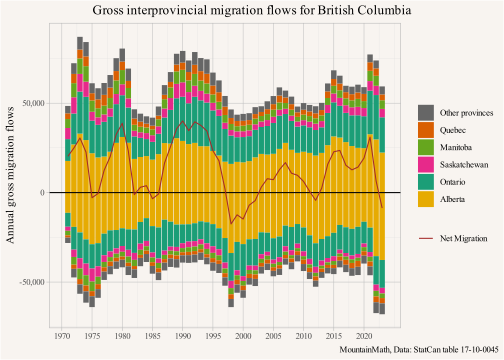
\includegraphics{index_files/mediabag/index_files/figure-pdf/fig-bc-interprovincial-migration-1.pdf}

}

\caption{\label{fig-bc-interprovincial-migration}Gross interprovincial
migration flows for British Columbia}

\end{figure}%

Interprovincial flows for BC are almost always dominated by what's
happening in Alberta (and usually more about oil prices than housing
prices).

When looking more broadly at gross out-flows, we can also incorporate
out-flows to other countries. StatCan estimated that 67,994 left BC for
other provinces in 2023, with another whopping 134,257 leaving BC for
other countries, 115,381 of which were non-permanent residents and
18,876 people emigrated. That's a lot of people leaving, but there are
also a lot of people moving to BC. And those international outflows are
more than offset by international inflows as illustrated in
Figure~\ref{fig-bc-interprovincial-external-migration}. For simplicity,
and for data availability, we are condensing the non-permanent resident
flows into net flows.

\begin{figure}[H]

\centering{

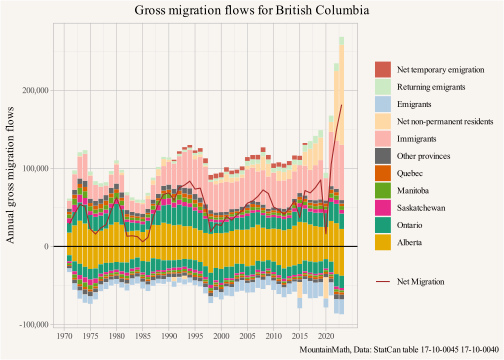
\includegraphics{index_files/mediabag/index_files/figure-pdf/fig-bc-interprovincial-external-migration-1.pdf}

}

\caption{\label{fig-bc-interprovincial-external-migration}Gross
interprovincial and external migration flows for British Columbia}

\end{figure}%

The pandemic effect and subsequent boom in non-permanent resident
population\footnote{There is a lot of misunderstanding about the nature
  of the increase in non-permanent residents out there, net
  non-permanent residents acts very differently from e.g.~increases in
  immigration. The data generation process for net non-permanent
  residents act essentially like a derivative and tends to zero absent
  of policy changes, but can temporarily rise (or fall) when hiring caps
  or student visa policies are changed.}, as well as changes to
permanent resident quotas, come out much more strongly here. So in total
450,106 people moved to BC in 2023, and 86,870 left BC, for a net
increase due to migration of 363,236 people. Rounding this out, because
population change is the sum of net migration + births - deaths, we can
see that even more 41,019 people were born in BC at the same time that
-44,122 died. Looking at only births and deaths leaves us with a net
decrease of 3,103. In other words, the ``natural population growth'' we
would see without net migration turned negative in the last couple of
years, as shown in Figure~\ref{fig-natural-population-growth}.

\begin{figure}[H]

\centering{

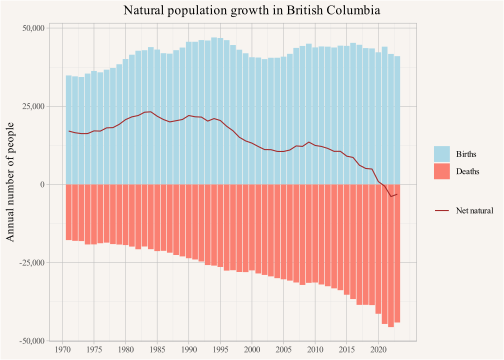
\includegraphics{index_files/mediabag/index_files/figure-pdf/fig-natural-population-growth-1.pdf}

}

\caption{\label{fig-natural-population-growth}Natural population growth
in British Columbia}

\end{figure}%

\section{Housing as a Reason for
Move}\label{housing-as-a-reason-for-move}

Back to housing and moves! Housing has long been one of the most
important reasons that people make local moves. But it's less often
considered a reason for longer-distance moves, especially between
regions or provinces. We can get a glimpse of this pattern with the
``reason for move'' data from the Canada Housing Survey.
Figure~\ref{fig-reason-for-last-move} shows the reasons people gave for
moving within or between cities.\footnote{While municipalities are
  sometimes similar to metro areas, e.g.~Calgary, Edmonton, or Winnipeg,
  there are important examples where they differ substantially and moves
  between municipalities are happening at high rates within the same
  metro area, e.g.~Vancouver, Toronto, or Montréal.} Using municipal
boundaries isn't ideal for distinguishing between short moves and
long-distance migration, insofar as some metro areas contain lots of
municipalities (e.g.~Vancouver), mixing short distance moves into our
``between city'' figure. But we can see the split emerging, with
employment a leading reason for ``between city'' moves, while housing
definitely dominates for ``within city'' moves.

\begin{figure}[H]

\centering{

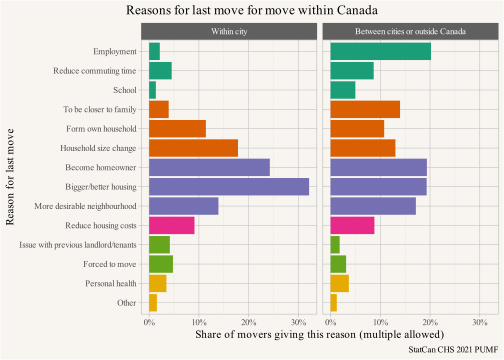
\includegraphics{index_files/mediabag/index_files/figure-pdf/fig-reason-for-last-move-1.pdf}

}

\caption{\label{fig-reason-for-last-move}Reasons given for moving within
a municipality or between municipalities, including from abroad.
Respondants could give multiple reasons.}

\end{figure}%

It's worth noting here that moves are pretty common, and mostly
positive. That is, people mostly move to somewhere they want to be more
than where they used to live. When this flips (as with forced moves) is
when we become concerned. Moving to ``reduce housing costs'' is a bit of
an edge case in this categorization.

Interestingly, when we look at the specifics of moving to ``reduce
housing costs'', the prevalence as a reason for move is similar for
within city and between city moves. But it's important to note that
reasons for move clearly overlap (and people could choose multiple
reasons for their move). For a given budget, people could think of
themselves as moving to a cheaper place both because it offered
``homeownership'' opportunities, ``bigger/better housing'' and/or
``reduced housing costs''. Overall we get some support for the idea that
housing matters for short distance moves and increasingly also for
longer-distance ones - even if not quite to the same level. That said,
if we focus only on why people chose one particular place to live, we
can miss why they didn't choose other places. Thinking about this at a
provincial level, we know lots of people are thinking of leaving BC
because of housing costs, but we don't have good data (beyond anecdotal)
about how many people are avoiding coming to BC because of housing
costs. We do know, thanks to a
\href{https://www.cbc.ca/news/canada/calgary/poll-canadians-comfortable-living-1.6302361}{CBC/Maru
study} from December of 2021, that BC is most often identified as a
province where Canadians would feel ``comfortable'' living.\footnote{The
  \href{https://www.marugroup.net/public-opinion-polls/canada/living-comfortably-elsewhere}{survey
  of Maru Voice Canada members} is structured similarly to the Angus
  Reid Forum, drawing upon an opt-in on-line panel in a manner meant to
  reflect the Canadian population as a whole} That suggests a lot of
untapped interest in moving to BC. We're really interested in how much
perceived housing costs inhibit people from making the move, and this
underlies a great deal of the uncertainty regarding our ability to
forecast into the future. How many people would come to BC if we made
housing cheaper?

\section{Metro Areas}\label{metro-areas}

Ultimately, people mostly don't move because they want to live in a
particular province. You don't move to live in BC, but instead to live
in or near Vancouver, or Victoria, or Kelowna. Correspondingly, what
we're really interested in when we look at longer distance migration is
the metropolitan level.

We've actually looked at various claims of people leaving Metro
Vancouver a lot over the years (Lasuter 2016; von Bergmann 2017a, 2017b)
which were mostly the result of poor understanding of data and
demographics, and we have also quantified the in and outflows of people
from Vancouver and other metro areas. (von Bergmann 2018; von Bergmann
and Lauster 2020, 2019). But the notion that lots of people are fleeing
Vancouver is remarkably persistent, and often housing costs are thought
to be behind the imagined exodus. The recent Angus Reid survey results
return us to this notion, but also provide seemingly surprising evidence
against it. That is, Metro Vancouver is not the place in BC where most
people are thinking of leaving the province over housing costs.

So how does Metro Vancouver compare to other Census Metropolitan Areas
(CMAs) in terms of its outflows? Do we see a larger proportion of the
population leaving each year than elsewhere? We start by looking at
outflows to other parts of Canada, adding in emigrants as a separate
category but suppressing the more volatile non-permanent residents.

Figure~\ref{fig-metro-leaving-rates_2021} shows the latest available
data, for the July 2021 to 2022 time frame (using 2021 CMA boundaries).

\begin{figure}[H]

\centering{

\includegraphics{index_files/mediabag/index_files/figure-pdf/fig-metro-leaving-rates_2021-1.pdf}

}

\caption{\label{fig-metro-leaving-rates_2021}Share of population leaving
metro area each year for other parts of Canada and emigrants}

\end{figure}%

Metro Vancouver rounds out the major metropolitan areas with the lowest
proportion of their populations joining an outflow, at less than 3\%. By
contrast, other BC metropolitan areas show up in the middle of the
distribution (Victoria) and among the most outwardly mobile, exceeding
4\% (Abbotsford - Mission and Kelowna). In effect, the cheaper places
tend to see more people leave. Single year fluctuations can mask longer
trends, so it's good to also check 5-year averages to smooth out annual
bumps. Overall, the July 2016 to 2021 averages (on 2016 CMA boundaries)
look quite similar, as shown in Figure~\ref{fig-metro-leaving-rates}..

\begin{figure}[H]

\centering{

\includegraphics{index_files/mediabag/index_files/figure-pdf/fig-metro-leaving-rates-1.pdf}

}

\caption{\label{fig-metro-leaving-rates}Share of population leaving
metro area between 2016 and 2021 for other parts of Canada and
emigrants}

\end{figure}%

Even averaged over the long-term, people leave Vancouver at relatively
low rates compared to other metro areas. Indeed, Vancouver moves into
the second spot in terms of retaining its residents, just after
Montréal. And if we ignored emigrants Vancouver would take the top spot.
This might seem counter-intuitive at first. Why do we hear so much about
people leaving Vancouver over housing if so few people are leaving?

Importantly, the people that show up here have generally already found
some sort of housing. They might not be happy with it. But Vancouver
overall is a nice place to live, so people don't want to leave. And
generally speaking, they don't. But when they do leave, they make sure
we hear about it. And it's probably increasingly because of housing.

\section{Migration by age group}\label{migration-by-age-group}

Unhappiness with housing in Vancouver tracks pretty well with age.
Migration and mobility track with age as well. Unfortunately we don't
have the age breakdown for gross migration flows, but we can look at net
migration by age group. Figure~\ref{fig-metro-van-net-migration-age}
looks at intra- and inter-provincial net migration for Metro Vancouver.

\begin{figure}[H]

\centering{

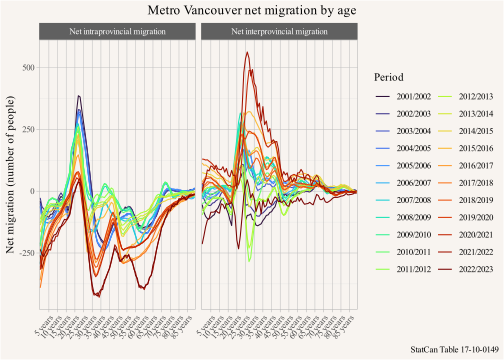
\includegraphics{index_files/mediabag/index_files/figure-pdf/fig-metro-van-net-migration-age-1.pdf}

}

\caption{\label{fig-metro-van-net-migration-age}Net migration by age
group for Metro Vancouver, focusing on intra- and inter-provincial
movers}

\end{figure}%

For intraprovincial migration we see a clear trend of declining net
migration across all age groups, with on net increasingly more people
leaving than arriving from other parts of the province. Metro Vancouver
still (just barely) absorbs more young people of university age from
around the province than it sends back out. But in all other age ranges,
more people leave for other parts of the province than arrive from those
parts. The inter-provincial patterns are more volatile, and more driven
by economic conditions between the provinces. Looking back at our
reasons for moving data, with housing being more important for more
local moves and employment related reasons more important for longer
distance moves, this is consistent with the notion that housing is
increasingly interfering with people's movements across regions.

Lastly, Figure~\ref{fig-metro-age-migration} compares net migration
patterns by age across selected metro areas for recent time periods.

\begin{figure}[H]

\centering{

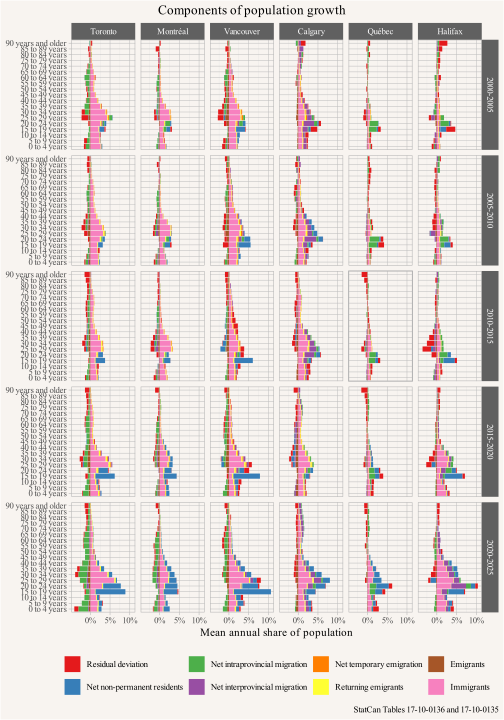
\includegraphics{index_files/mediabag/index_files/figure-pdf/fig-metro-age-migration-1.pdf}

}

\caption{\label{fig-metro-age-migration}Net migration by age group for
select metro areas and time periods.}

\end{figure}%

Here we averaged over (roughly) 5 year periods to smooth out the data
and simplify the presentation. Different metro areas show distinct
migration patterns, with e.g.~Toronto, Vancouver and Montréal showing
significant net intra-provincial out-migration (in green), acting as
\emph{arrival cities} for their provinces. All three CMAs also show an
increase in net intraprovincial out-migration over time, only somewhat
suppressed for young adults ages, likely by the strong pull of their
universities.

\section{Takeaway}\label{takeaway}

It's great to see more data on housing costs as a factor in people's
thinking about moves, especially for longer distances. That said the
data can still be tricky to interpret, and ``moving to another
province'', as in the Angus Reid survey, doesn't constitute a long move
for those living near borders. In conjunction with data on actual moves
and reasons given for moves, we can see some support for the idea that
housing costs are increasingly driving migration patterns. On the other
hand, high housing costs also reflect migration and indicate that people
want to live in a place.

Even though really expensive regions, like Metro Vancouver, don't see
that much out-migration, many of the people who do leave likely do so in
part for housing reasons. But there are a lot of reasons people move. We
should also keep an eye on net migration patterns, insofar as many of
the people who would like to come to places like Metro Vancouver are
probably feeling shut out by housing costs. It's hard to get at this
directly insofar as we seldom ask everyone about where they'd like to
be. But when we do, Canadians often say BC.

And we agree. BC, and particularly Metro Vancouver, is a nice place to
live. It'd be even nicer if it was a little more welcoming. Adding more
housing is how we get there.

As usual, the code for this post is
\href{https://github.com/mountainMath/mountain_doodles/blob/main/posts/2024-06-11-migration-and-housing-costs/index.qmd}{available
on GitHub} for anyone to reproduce or adapt for their own purposes.

\phantomsection\label{refs}
\begin{CSLReferences}{1}{0}
\bibitem[\citeproctext]{ref-lifeblood.2016}
Lasuter, Nathan. 2016. {``Is the Lifeblood of Vancouver Leaving?''}
\url{https://homefreesociology.com/2016/02/12/is-the-lifeblood-of-vancouver-leaving/}.

\bibitem[\citeproctext]{ref-lifeblood.2017}
von Bergmann, Jens. 2017a. {``Lifeblood.''}
\url{https://doodles.mountainmath.ca/posts/2017-05-16-lifeblood/}.

\bibitem[\citeproctext]{ref-millennials-redux.2017}
---------. 2017b. {``Millennials {Redux}.''}
\url{https://doodles.mountainmath.ca/posts/2017-08-06-millennials-redux/}.

\bibitem[\citeproctext]{ref-gross-migration.2018}
---------. 2018. {``Gross Migration.''}
\url{https://doodles.mountainmath.ca/posts/2018-08-16-gross-migration/}.

\bibitem[\citeproctext]{ref-there-is-no-brain-drain-but-there-might-be-zombies.2019}
von Bergmann, Jens, and Nathan Lauster. 2019. {``There Is No {Brain}
{Drain,} but There Might Be {Zombies}.''}
\url{https://doodles.mountainmath.ca/posts/2019-02-03-there-is-no-brain-drain-but-there-might-be-zombies/}.

\bibitem[\citeproctext]{ref-keeping-the-leavers.2020}
---------. 2020. {``Keeping the {Leavers}.''}
\url{https://doodles.mountainmath.ca/posts/2020-08-27-keeping-the-leavers/}.

\end{CSLReferences}



\end{document}
